\section{Trigger System Validation with Beam}
\label{sec:validation}

When beam operations started, the Trigger System validation was completed as part of the entire CLAS12 detector commissioning. This section describes the trigger validation procedures. 

\subsection{``Random Trigger" Validation Procedure}
\label{sec:validation_random}

The ultimate validation of the trigger is done using the so-called ``Random Trigger'' (RT) runs. RT runs are special runs where the event readout is initiated not by the trigger logic, but by an external random generator that can be tuned to the desired frequency. Most of the events in the RT runs do not contain any tracks, however, a small fraction of the events will have real particles that were reconstructed because particle accidentally fell in the readout window that was initiated by the random generator. In the event readout, in addition to various data banks from DAQ system, the trigger decisions are stored as well (see Section \ref{sec:trigger_in_datastream}).

These accidental ``good'' events are used to check whether the desired trigger bit in the Stage 3 32-bit trigger mask was set by the trigger logic. In case it is not set, information from the Stage 1 and Stage 2 trigger is available to analyse the possible reasons for the inefficiency.

\begin{figure}[!htb]
	\centering
	\subfloat[]{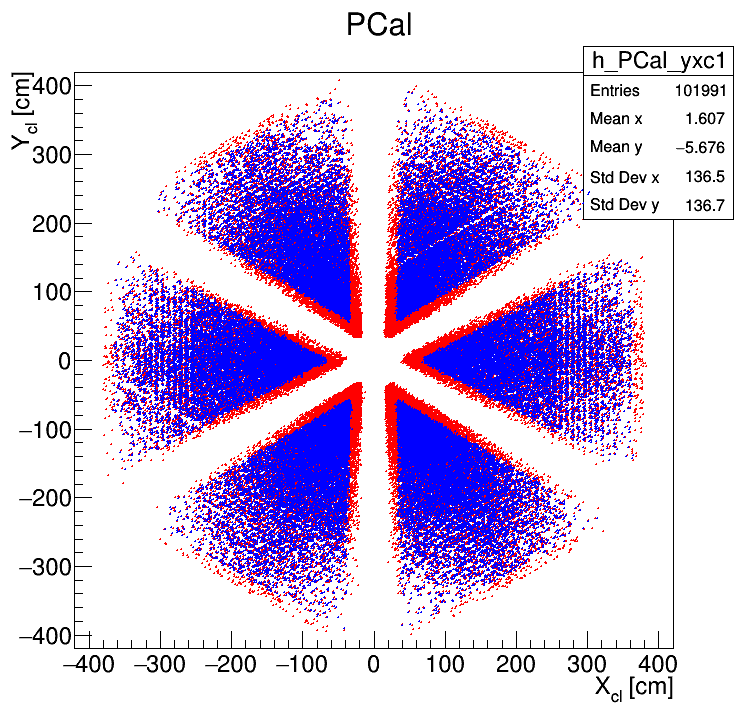
\includegraphics[width=0.24\textwidth]{img/PCal_Fiducials_4878.png}}
	\subfloat[]{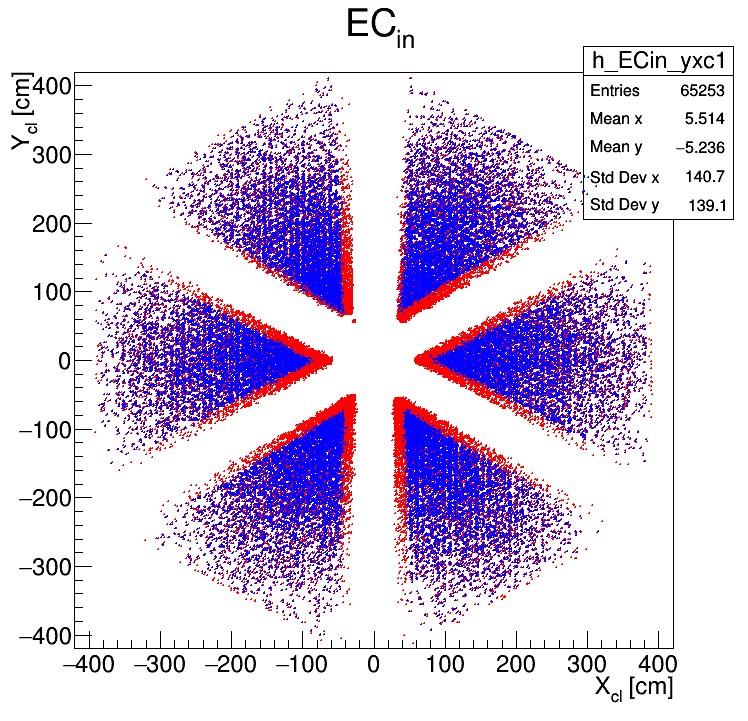
\includegraphics[width=0.24\textwidth]{img/ECin_Fiducials_4878.png}}
	\caption{Distribution of cluster coordinates of PCAL (left) and EC\_{in} (right).
		scatter plot in Red shows all events, while blue scatter plot show events where cluster
		is in the fiducial region of the calorimeter (about 15 cm away from the edges).}
	\label{fig:pcal_clusters}
\end{figure}

The technique of the trigger validation is as follows. The trigger logic is configured exactly as it will be set in an experiment, but it runs in ``tagging mode'', reporting trigger decisions into the data stream for every randomly generated event. After several hours of running we collect at least 100 million events.

After the data is processed and the events are reconstructed, we select subset of events with correct trigger time. It is done using FADC spectra for detectors participating in the trigger logic. We need to select events with the FADC spectra similar to the one in the data obtained using regular trigger. Fig. ~\ref{fig:htcc_fadc} (left) shows typical FADC pulses for the regular (not random) trigger, with pulse width below 50~ns. Reconstructing and analyzing the data obtained using random trigger, we select events with signal in the middle of the FADC window to make sure we do not have boundary effects when the signal region is selected. Based on the typical pulse shape, we ignore areas below 50~ns and above 150~ns (see Fig. ~\ref{fig:htcc_fadc} (right)).

\begin{figure}[!htb]
	\centering
	\subfloat[]{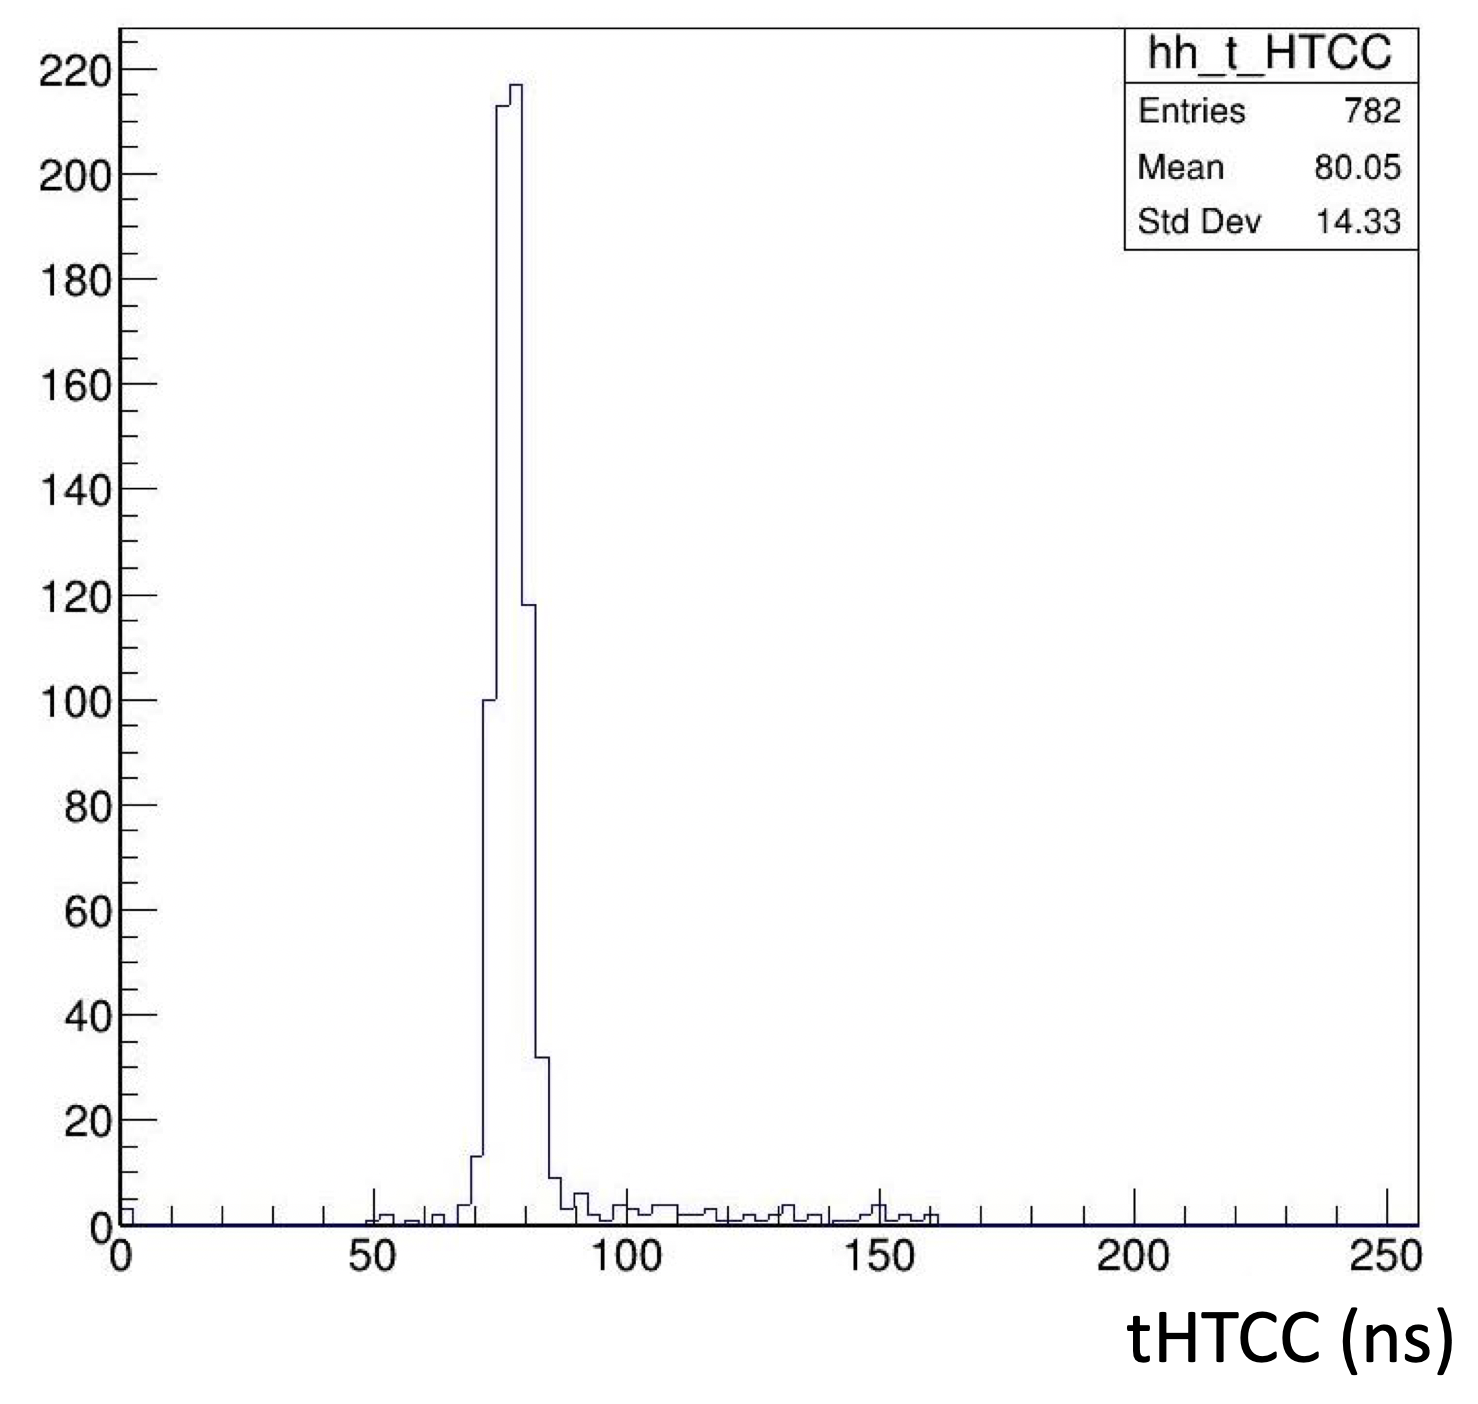
\includegraphics[width=0.24\textwidth]{img/htcc_fadc1.png}}
	\subfloat[]{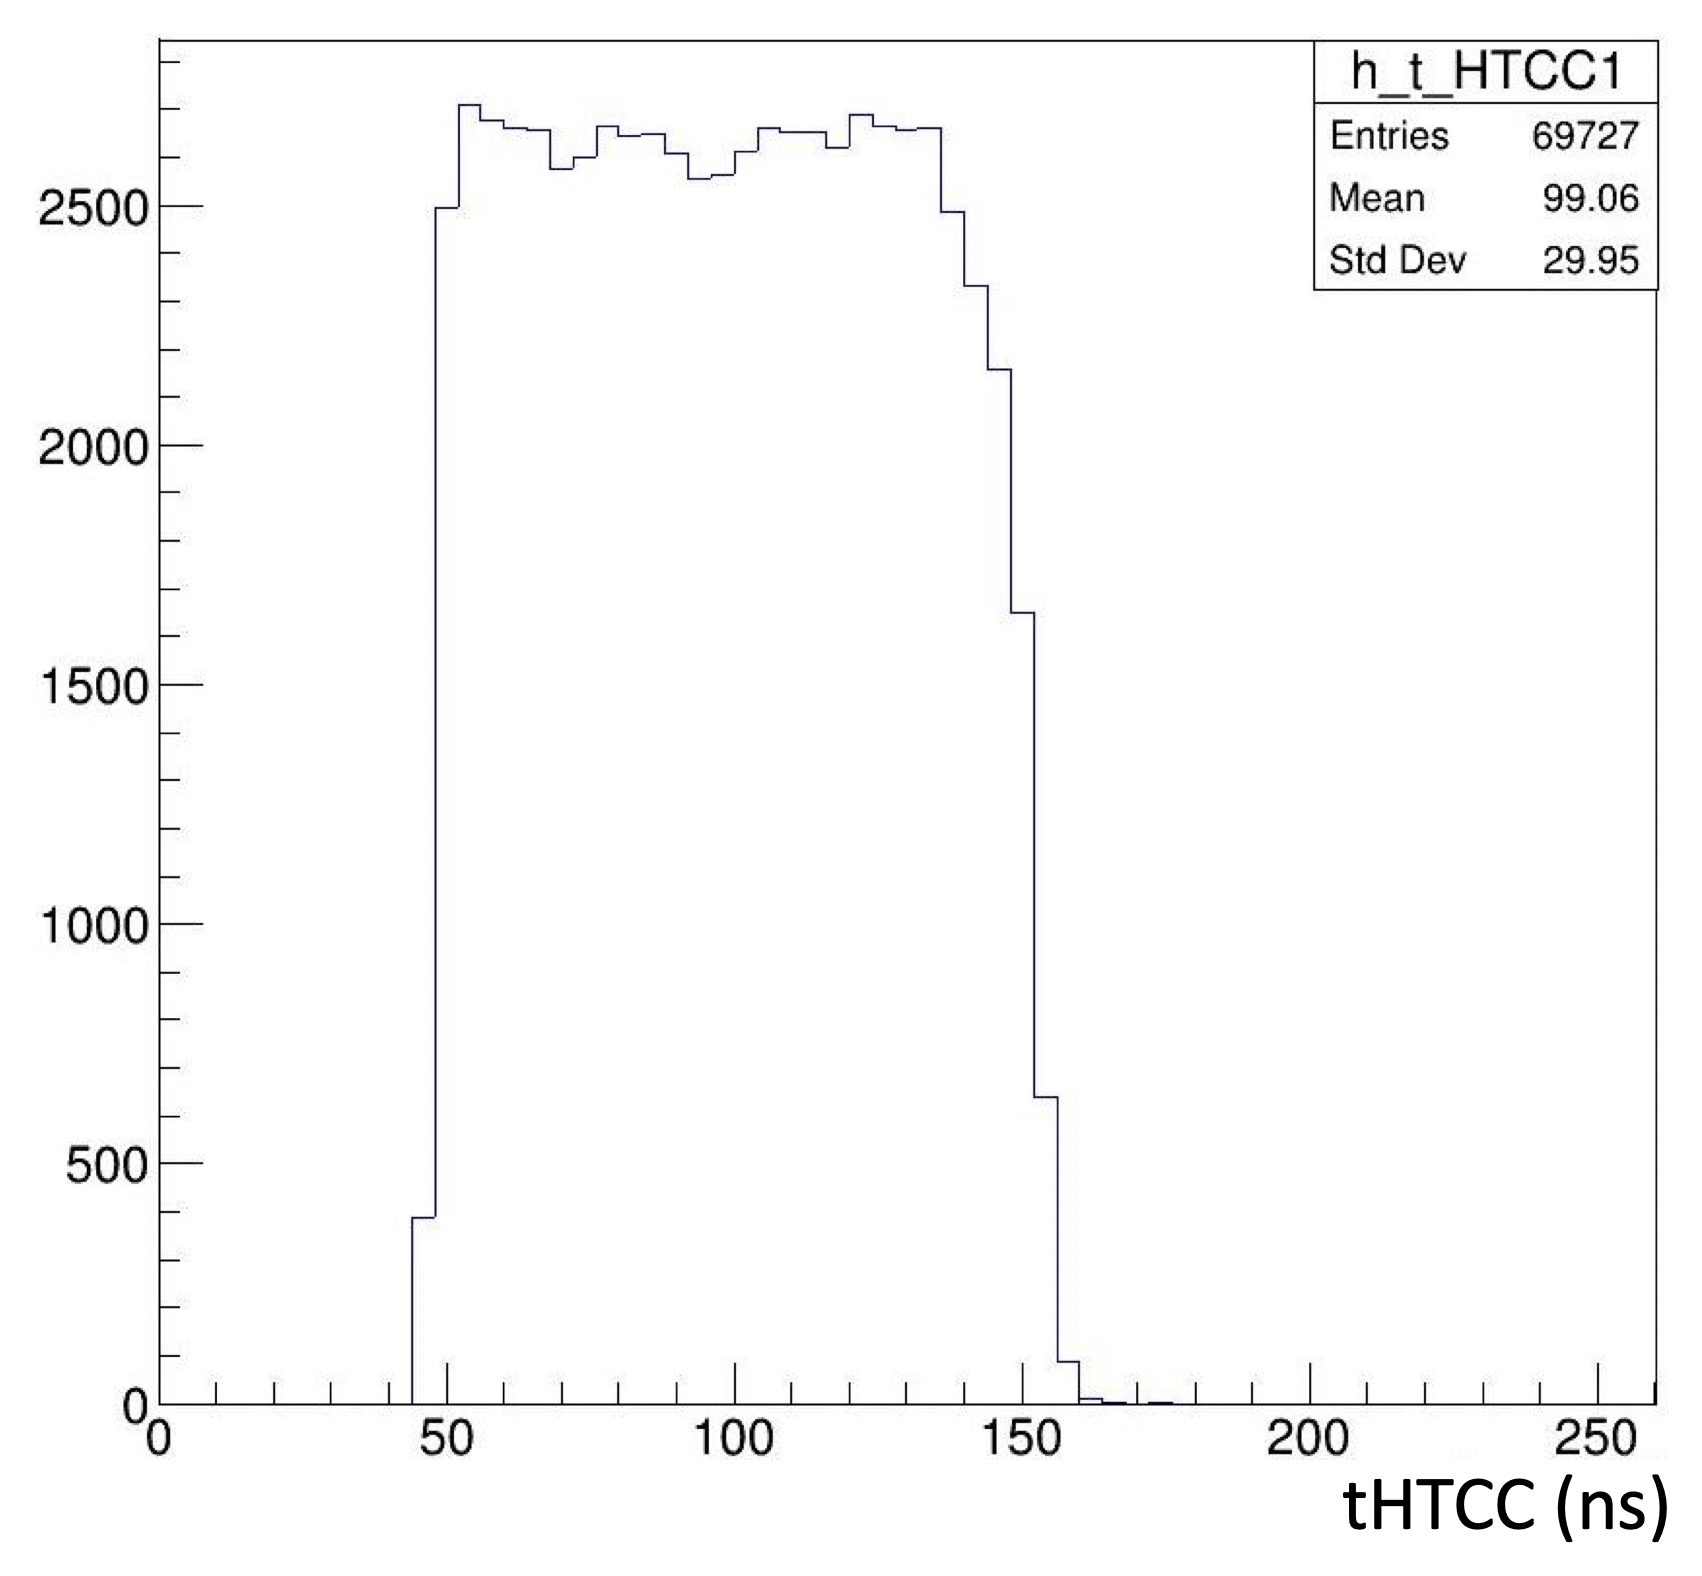
\includegraphics[width=0.24\textwidth]{img/htcc_fadc2.png}}
	\caption{HTCC FADC pulses: left - physics triggers, right - randon trigger. Plot was used to select ``good'' events from the random trigger runs, for such events FADC timing have to be at least 50 counts from both timing window edges to avoid boundary effects.}
	\label{fig:htcc_fadc}
\end{figure}

We typically find several thousands events that accidently fell into the correct trigger window. These events can be used to obtain the trigger efficiency and purity assuming that our off-line reconstruction software works correctly. It should be mentioned that correctly working of the off-line reconstruction is an important pre-requisite for complete trigger validation.


\subsection{Validation of the Electron Trigger}
\label{elctron_trigger_validation}
As a reminder the electron trigger logic uses responces from PCAL, EC, HTCC and DC (see eq. \ref{eq:em_trg_formula}), and as it was described in section \ref{sec:validation_random}, for trigger validation we have used a Random Trigger data. 
The $\mathrm{1^{st}}$ step in the validation of electron trigger is a selection of  events with ``clean electron''. The CLAS12 offline reconstruction software assignes PID to each reconstruction particle ({\color{Red} reference to offline recon.}) ( for electron PID=11) however in this studies we imposed additional cuts. 
In particular 
\begin{itemize}
 \item DC roads are optimized for tracks originating from the target, that is why in the offline analysis we have put a cut on the vertex ``Z'' coordinate to make sure the track originates from the target.
 \item Selected events where electron hits calorimeters (PCal and EC) in a fiducial region, to make sure the shower is fully reconstructed.
 \item Applied trigger condition cuts on offline cluster energies in the PCAL and EC, also on number of photoelectrons in HTCC.
\end{itemize}
After applying above mentioned cuts, for each of these electrons, we have checked whether the electron trigger bit is set for the corresponding sector. At the end the trigger efficiency is defined as the number of ``Bit  Set'' events over the number of all events with ``clean'' electron.
Both RG-A and RG-B experiments required to have a good (close to $100 \%$) trigger efficiency for electron above $\mathrm{2\;GeV}$. Since both PCAL and EC are sampling calorimeters, $\mathrm{2\;GeV}$ electrons will deposit only part (in average about $25\%$ in our case) of the the total energy. Then because of shower and light fluctuations some $\mathrm{2\;GeV}$ electrons will have less than $\mathrm{25\%}$ energy reconstructed in the calorimeters. Based on this, in the trigger we required the energy to be more than $\mathrm{300 \; MeV}$, which guarantee that more than $\mathrm{99\%}$ of $\mathrm{2\;GeV}$ electrons will deposit energy above the threshold.

\begin{figure}[!htb]
 \centering
 \subfloat[]{\label{fig:em_eff_Allcomponents}\grinp[width=0.25\tw]{img/All_components_65416544.pdf}}
 \subfloat[]{\label{fig:em_nphe_Miss}\grinp[width=0.25\tw]{img/nphe_missed1_65416544.pdf}}
 \caption{(a) Momentum distribution of ``Good electrons''. The brown distribution represents all ``Good electrons'', The blue histograms represents all events where the electron trigger bit was not set, the black histogram represent events, which doesn't have $\mathrm{EC}\times \mathrm{PCal}$ trigger bit, and the red one represent events that missed the electron trigger bit. (b) distribution of the number of photoelectrons for where the electron has more than $\mathrm{2\;GeV}$ energy and missed the HTCC trigger bit.}
 \label{fig:em_missed_events}
\end{figure}

Fig.\ref{fig:em_eff_Allcomponents} shows the momentum distributions of all ``Good'' electrons (in brown), electrons when electron trigger bit was not set  (in blue), when $\mathrm{EC}\times \mathrm{PCAL}$ bit was not set (in black), and red represents events when HTCC bit was not set. As one can see, above $\mathrm{2\; GeV}$ most of events have only HTCC bit missing.  Fig.\ref{fig:em_nphe_Miss} presents the distribution of the number of photoelectrons for events, which have no  HTCC trigger bit. As one can see about $\mathrm{90\%}$ of these events are    at the threshold region (reminder that in the trigger we used 2 photoelectron threshold).  The Trigger System has different from the offline reconstruction  precision of gains and pedestals values. ({\color{Red}probably Ben can comment what was the exact precision}) It could potentially create  such threshold related effects.

\begin{figure}[!htb]
 \centering
 \grinp[width=0.45\tw]{img/em_Efficiency_65416544.pdf}
 \caption{Trigger efficiency as a function of the electron momentum.}
 \label{fig:em_eff}
\end{figure}

The final efficiency is shown in the Fig.\ref{fig:em_eff}, where we can see that  the trigger efficiency is above $\mathrm{95\; \%}$
for electrons with momentum above $\mathrm{2\ GeV}$.



\subsection{Validation on beam during CLAS12 detector commissioning -  photoproduction trigger}

As described in section \ref{sec:photoproduction_trigger}, the CLAS12 photoproduction trigger requires the coincidence between one electron measured in the Forward Tagger detector, and two hadrons measured within the CLAS12 detector, in the forward or central part. The validation procedure aims to verify if, for a given event foreseeing one final-state electron in the FT acceptance and two or more hadrons scattered within the CLAS12 acceptance, the trigger system would recognize it properly, resulting in event readout. In order to validate the system with beam during commissioning, the following strategy was adopted. First, the $e^-$ detection by the FT was validated using Random Trigger runs. After this, the detection of single hadrons in CLAS12 was studied in special runs, were the only trigger source was the FT. Finally, the coincidence between the two systems was assessed.

\subsubsection{Validation of $e^-$ detection in FT}

A scattered electron in the Forward Tagger is identified as an electromagnetic shower in the Forward Tagger Calorimeter within a proper energy range, in time coincidence and geometrically matched to a hit in both layers of the Forward Tagger Hodoscope. The map providing the matching between the cluster seed position in the FT-Cal and the tiles position in the FT-Hodo was first derived by the nominal detector geometry, and then confirmed by Montecarlo simulations.

The identification of the scattered $e^-$ in the FT was validated through a similar procedure as the one adopted for the CLAS12 electron trigger discussed before, based on ``Random Trigger'' runs. Recorded events were processed through the standard CLAS12 reconstruction software and filtered, keeping only those with a reconstructed $e^-$ in the FT system. Since event readout was triggered by a random pulser, events with the reconstructed $e^-$ signal close to the margins of the readout window were also rejected.
For these events, the electromagnetic clusters found by the reconstruction software (``offline'' clusters) were compared to those reported by the trigger system and stored in the form of the trigger data banks.

The efficiency of the FT-Cal clustering algorithm in the trigger system was evaluated by comparing all ``offline'' clusters to those matched - in space and time - to an ``online'' one\footnote{The energy of ``offline'' clusters is properly corrected to account for electromagnetic shower leakage from the bak of the FT-Cal, while ``online'' clusters do not implement this. Therefore, for a given $e^-$ in the FT-Cal, there is a systematic difference between the two energies. This effect is properly taken into account when setting the energy range for $e^-$ detection in the trigger system, and does not affect the corresponding trigger efficiency.}. The efficiency was computed as:
\begin{equation}
\varepsilon=\frac{N_{trigger}}{N_{all}} \; ,
\end{equation}
where $N_{all}$ and $N_{trigger}$ are, respectively, the total number of ``offline'' clusters and the number of ``offline'' clusters matched to an ``online'' one.
The result is shown in Fig.~\ref{fig:FT_ClusterEfficiency}, reporting the FT trigger efficiency for electromagnetic clusters as a function of the corresponding corrected energy. Efficiency is higher than 97.5$\%$ in the full energy range of interest / 99.5$\%$ in the energy range above 1 GeV. The difference is mainly due to the fact that the clustering algorithm in the trigger system works on a 3x3 matrix of crystals, whereas this limitation doesn't hold in the offline reconstruction.
The efficiency of the FT-Cal / FT-Hodo matching algorithm was evaluated in a similar way, repeating previous calculation but considering only electromagnetic clusters associated to one hit in each FT-Hodo layer. The result is reported in Fig.~\ref{fig:FT_ClusterEfficiencyHODO}.

%%%%%%%%%%%%%%%%%%%%%%%%%%%%%%%%%%%%%%%%% F I G U R E %%%%%%%%%%%%%%%%%%%%%%%%%%%%%%%%%%%%%%%%%%
\begin{figure}[!htb]
 \centering
{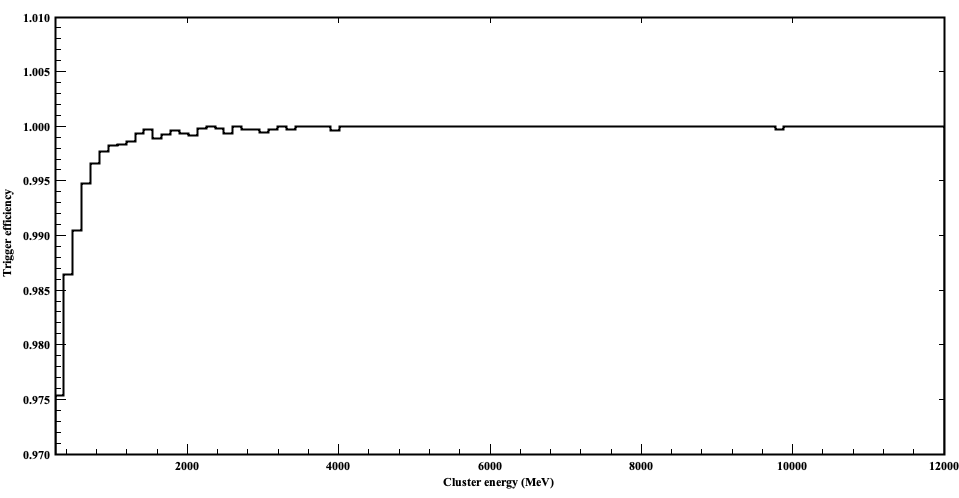
\includegraphics[width=.5\textwidth]{img/FT_ClusterEfficiency.png}}
 \caption{TODO: better figure, with errors (run 4288)}
 \label{fig:FT_ClusterEfficiency}
\end{figure}
%%%%%%%%%%%%%%%%%%%%%%%%%%%%%%%%%%%%%%%%% F I G U R E %%%%%%%%%%%%%%%%%%%%%%%%%%%%%%%%%%%%%%%%%%




\subsubsection{Validation of charged hadrons detection in CLAS12-FD}

The trigger system recognizes a charged hadron in the CLAS12 forward detector as a hit in the Forward Time-Of-Flight system (panel 1B) in time coincidence and geometrically matched to a hit in the U-bars of the Preshower Calorimeter, associated to a cluster with energy larger than a programmable threshold. The map providing the geometrical matching between FTOF counter and the PCAL U-bar was first derived by the nominal detector geometry, and then confirmed by Montecarlo simulations. To reduce the rate of random coincidences, the trigger system also requires the presence of a segment in 5 out of 6 drift chamber layers. The charged hadron identification algorithm was validated in special data-taking runs in which the Forward Tagger was the only enabled event readout source. In these runs, the trigger system was configured to report in the output trigger bank the presence of a charged hadron in any CLAS12-FD sector, as defined before. 

Recorded events were processed through standard reconstruction software and filtered, keeping only those with a well reconstructed charged track measured in CLAS12-FD. The track was required to be within the nominal acceptance of CLAS12 PCAL, and a momentum threshold of 300 MeV/c was applied. The trigger system efficiency was evaluated by comparing all reconstructed tracks to the tracks recognized by the trigger system. During commissioning, the efficiency was evaluated as a function of different observables, such as the energy deposited in the FTOF counters and in the PCAL, and the topology of the geometrical matching window. Trigger parameters were individually tuned to maximize the trigger efficiency. In the final configuration, an energy threshold of 2 MeV and 10 MeV for the FTOF counters and PCAL clusters was selected.  The result is reported in Fig.~\ref{fig:FD_TrackEfficiency}, showing the CLAS12-FD trigger efficiency for charged hadrons as a function of the track momentum. The efficiency is larger than 99$\%$ in the full momentum range, the inefficiency being dominated by threshold effects for the PCAL clusters.

%%%%%%%%%%%%%%%%%%%%%%%%%%%%%%%%%%%%%%%%% F I G U R E %%%%%%%%%%%%%%%%%%%%%%%%%%%%%%%%%%%%%%%%%%
\begin{figure}[!htb]
 \centering
{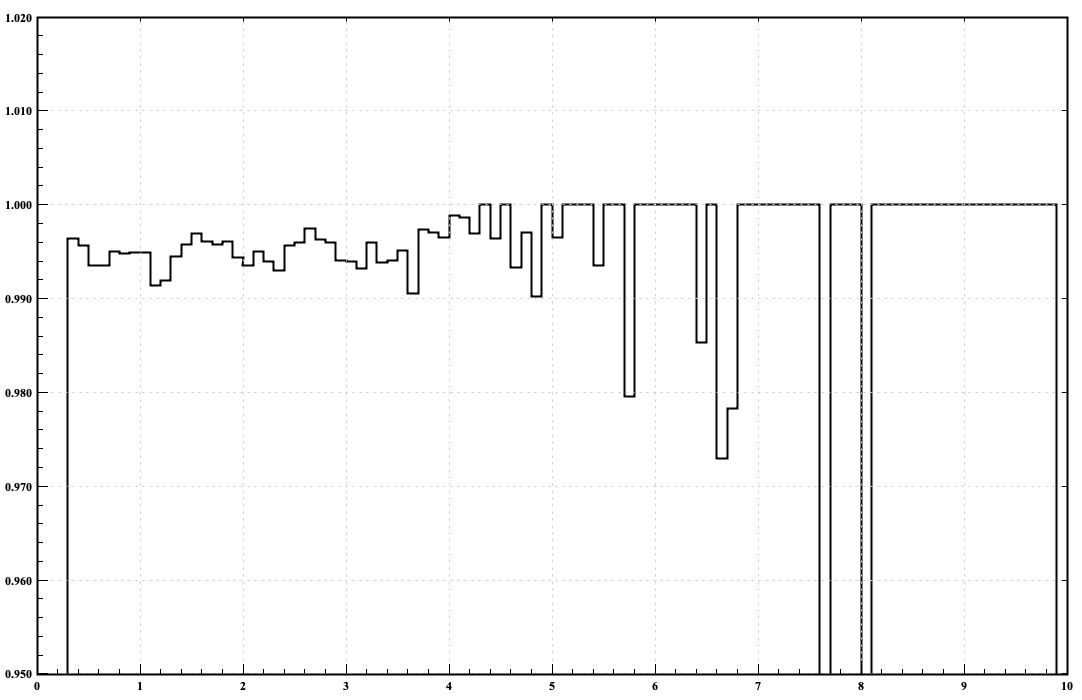
\includegraphics[width=.5\textwidth]{img/FD_TrackEfficiency.png}}
 \caption{TODO: better figure, with errors - run 5049-5050 (run4)}
 \label{fig:FD_TrackEfficiency}
\end{figure}
%%%%%%%%%%%%%%%%%%%%%%%%%%%%%%%%%%%%%%%%% F I G U R E %%%%%%%%%%%%%%%%%%%%%%%%%%%%%%%%%%%%%%%%%%



\subsubsection{Validation of charged hadron detection in CLAS12-CD}

The trigger system recognizes a charged hadron in the CLAS12 central detector as a hit in the Time-Of-Flight system (panel 1B) in time coincidence and geometrically matched to a hit in the U-bars of the Preshower Calorimeter.





\subsection{Drift Chamber-Based Trigger Components and Data-Based Dictionary}
\label{dc_dictionary}

The road dictionary for the DCs used within the Trigger System was initially generated using a fast Monte Carlo approach, where positive and negative particles in a selected momentum and angular range were randomly generated, tracked in the CLAS12 magnetic field using the CLAS ``swimmer'' developed for the offline reconstruction based on a 4th-order Runge-Kutta approach, and projected onto the DC wire planes to determine the hit position and therefore the DC wire IDs. This method has intrinsic limitation because of the approximation done in tracking the particle through the detector that does not include energy loss, multiple scattering, or other effects due to the particle interactions with the detector material.

To overcome these limitations, roads were also generated from full GEANT4 simulations of the CLAS12 detector based on the GEMC package as described in Section \ref{simulated_data_preparation}. This provides an accurate description of the relevant materials the particles travel through, resulting in a more accurate road dictionary at the expenses of a significantly higher computing time to generate the same size dictionary.

The effectiveness of these two approaches was tested by using real tracks from beam data to evaluate the completeness of the dictionaries, i.e. the fraction of tracks for which a matching road is found. This study indicated that very large statistics is needed in the dictionary-making to populate specific regions of the phase space.

As a third alternative approach, dictionaries were also produced from real tracks from beam data: in this case dictionaries with very large statistics can be produced in limited computing time with the advantage of the best accuracy in accounting both for particle interaction in matter and for the real detector geometry. These were the dictionaries that were used in the final trigger implementation.




\subsection{Final Validation Before Experiment Start-up}

After the CLAS12 detector was commissioned and the Trigger System components were validated, we still have to execute our validation processes for the entire system at the begining of every experiment. This is necessary because different experiments request configuration changes in the Trigger System, that take advantage of its flexibility. Also, we apply firmware changes occasionally to improve the Trigger System components based on our previous experience, and then changes have to be validated. The final Trigger System validation is performed by taking beam data with a random trigger (see Section ~\ref{sec:validation_random}).

The final trigger validation procedure was executed several times during the first year of CLAS12 experiments and was proven to be very useful: bugs in the trigger firmware were found and fixed, and the trigger configuration parameters were optimized. On one occasion a firmware bug was introduced into the PCAL Stage 1 trigger logic during the firmware update that was expected to be small and simple. The final validation procedure revealed an irregularity in the spacial distribution of clusters (see Fig.~\ref{fig:PCAL_bug_data}) (it also shows one CLAS12 sector is missing but this was another problem unrelated to the Trigger System). Since the PCAL Stage 1 trigger firmware is implemented in C++/HLS, the GEANT4 data sample was reprocessed through the C++ firmware implementation (see Fig.~\ref{fig:PCAL_bug_hls}), and the problem was confirmed and subsequently found and fixed. The firmware was recompiled and reloaded, and the final trigger validation was repeated showing that the problem was fixed. It took only several hours between finding the problem and being ready to run again. Every experiment in CLAS12 begins with a complete Trigger System validation. 

\begin{figure}[hbt]
	\centering
	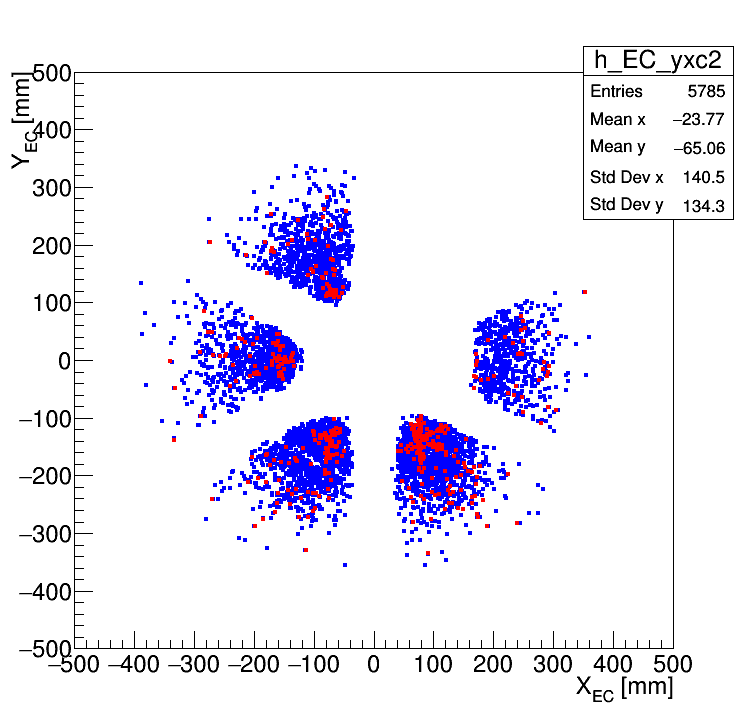
\includegraphics[width=1.0\columnwidth,keepaspectratio]{img/PCAL_bug_data.png}
	\caption{PCAL bug in beam data. Red crosses inside blue areas coresponds to trigger inefficiency, it was discovered during beam data processing.}
	\label{fig:PCAL_bug_data}
\end{figure}

\begin{figure}[hbt]
	\centering
	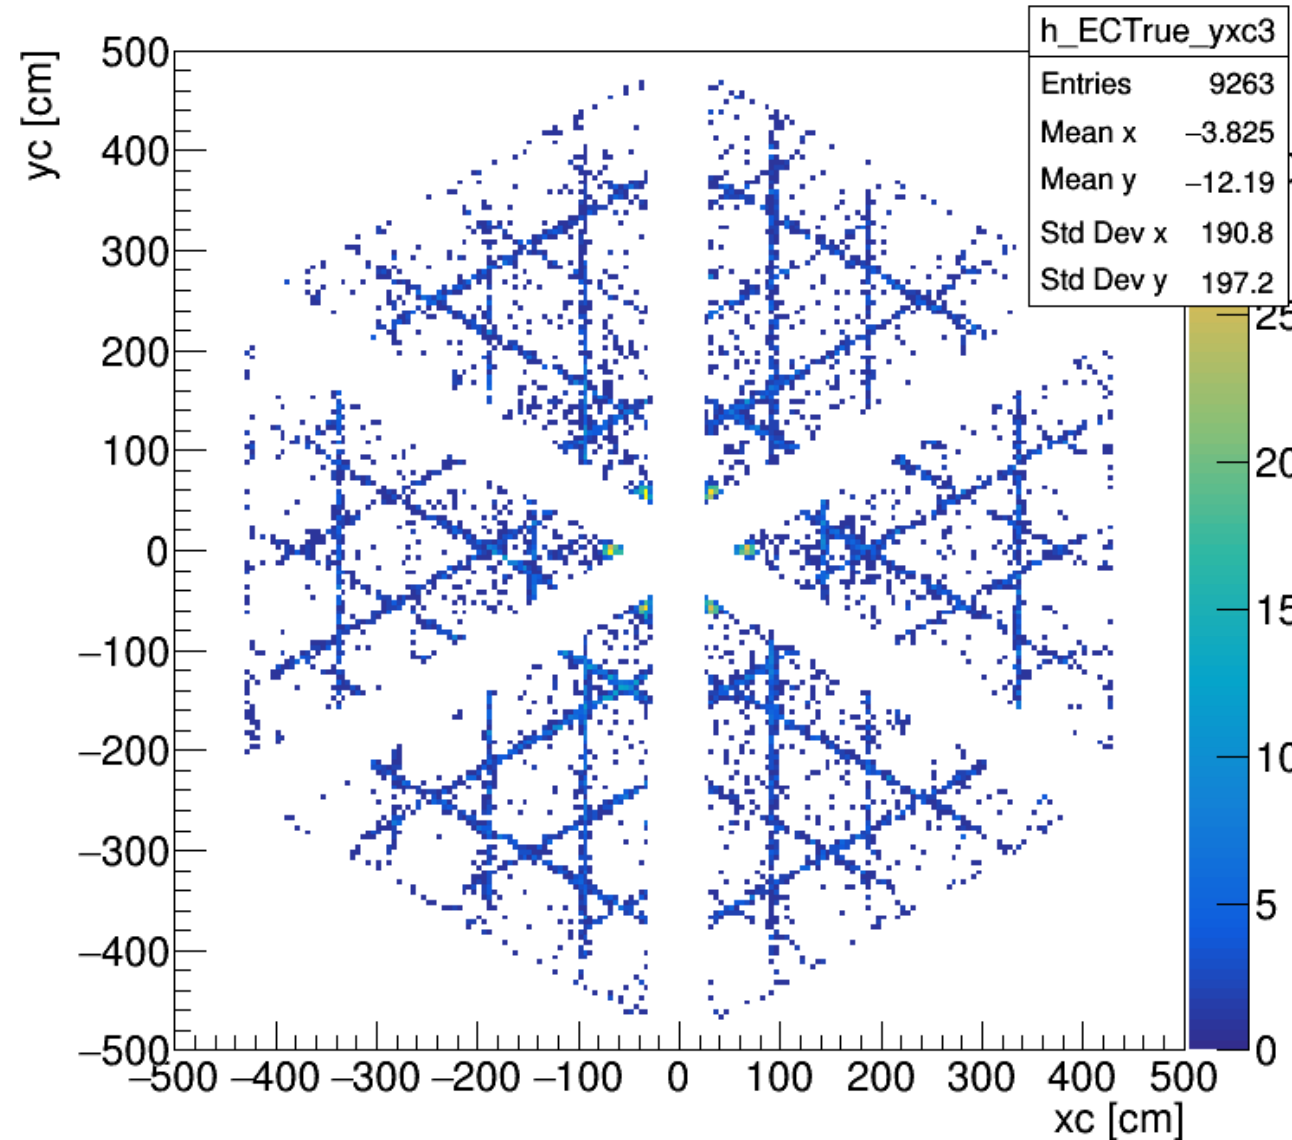
\includegraphics[width=1.0\columnwidth,keepaspectratio]{img/PCAL_bug_hls.png}
	\caption{PCAL bug in GEANT4 simulation. Blue lines corresponds to trigger inefficiency. It is visible much better in simulation then in beam data, and points to exact problem.}
	\label{fig:PCAL_bug_hls}
\end{figure}

